\documentclass[apj, revtex4]{emulateapj}

%%%%% AUTHORS - PLACE YOUR OWN PACKAGES HERE %%%%%
%\usepackage[colorlinks,urlcolor=blue,citecolor=blue,linkcolor=blue]{hyperref}
%\usepackage{color}
%\usepackage{graphicx}
%\usepackage{amsmath}	% Advanced maths commands
%\usepackage{amssymb}	% Extra maths symbols
%\usepackage{mathrsfs}	% Extra extra math symbols
%\usepackage{natbib}
%\usepackage[colorlinks,urlcolor=magenta,citecolor=blue,linkcolor=blue]{hyperref}
%\usepackage{multirow}
%\usepackage{etoolbox}
%\usepackage{subfig}
%\usepackage{microtype}
%\usepackage{listings}

\usepackage{epsf}
\usepackage{color}
\usepackage{amsmath}
\usepackage{graphicx}
\usepackage[colorlinks,urlcolor=magenta,citecolor=blue,linkcolor=blue]{hyperref}
\usepackage{threeparttable}
\usepackage{multirow}
\usepackage{natbib}
\usepackage{etoolbox}
\usepackage{longtable}

\bibliographystyle{apj}
\citestyle{aa}

%%%%% AUTHORS - PLACE YOUR OWN COMMANDS HERE %%%%%
%%% Fields %%%
\newcommand{\hdf}{HDF-N}
\newcommand{\hdfn}{HDF-N}
\newcommand{\hdfs}{HDF-S}
\newcommand{\cdfs}{CDF-S}

%%% Telescopes %%%
\newcommand{\hst}{\textit{HST}}
\newcommand{\iras}{\textit{IRAS}}
\newcommand{\iso}{\textit{ISO}}
\newcommand{\spitzer}{\textit{Spitzer}}
\newcommand{\sirtf}{\textit{Spitzer}}
\newcommand{\chandra}{\textit{Chandra}}
\newcommand{\planck}{\textit{Planck}}

%%% Filters %%%
\newcommand{\wfu}{\hbox{$\mathrm{U}_{300}$}}
\newcommand{\wfb}{\hbox{$\mathrm{B}_{450}$}}
\newcommand{\wfv}{\hbox{$\mathrm{V}_{606}$}}
\newcommand{\wfi}{\hbox{$\mathrm{I}_{814}$}}
\newcommand{\acsb}{\hbox{$\mathrm{B}_{435}$}}
\newcommand{\acsv}{\hbox{$\mathrm{V}_{606}$}}
\newcommand{\acsi}{\hbox{$i_{775}$}}
\newcommand{\acsz}{\hbox{$z_{850}$}}
\newcommand{\nicj}{\hbox{$\mathrm{J}_{110}$}}
\newcommand{\nich}{\hbox{$\mathrm{H}_{160}$}}
\newcommand{\wfcy}{\hbox{$\mathrm{Y}_{105}$}}
\newcommand{\wfcj}{\hbox{$\mathrm{J}_{125}$}}
%\newcommand{\wfcj}{\hbox{$J_{110}$}}
\newcommand{\wfch}{\hbox{$\mathrm{H}_{160}$}}
\newcommand{\sdssu}{\hbox{$u$}}
\newcommand{\sdssg}{\hbox{$g$}}
\newcommand{\sdssr}{\hbox{$r$}}
\newcommand{\sdssi}{\hbox{$i$}}
\newcommand{\sdssz}{\hbox{$z$}}
\newcommand{\mone}{\hbox{$[3.6]$}}
\newcommand{\mtwo}{\hbox{$[4.5]$}}
\newcommand{\mthree}{\hbox{$[5.8]$}}
\newcommand{\mfour}{\hbox{$[8.0]$}}
%\newcommand{\mone}{\hbox{$[3.6\mu\mathrm{m}]$}}
%\newcommand{\mtwo}{\hbox{$[4.5\mu\mathrm{m}]$}}
%\newcommand{\mthree}{\hbox{$[5.8\mu\mathrm{m}]$}}
%\newcommand{\mfour}{\hbox{$[8.0\mu\mathrm{m}]$}}

%%% Astronomy Abreviations %%%
\newcommand{\mstar}{\hbox{M$_{\star}$}}
\newcommand{\lstar}{\hbox{L$_{\star}$}}
\newcommand{\Msol}{\hbox{$\mathrm{M}_\odot$}}
\newcommand{\msol}{\hbox{$\mathrm{M}_\odot$}}
\newcommand{\Zsol}{\hbox{$Z_\odot$}}
\newcommand{\zsol}{\hbox{$Z_\odot$}}
\newcommand{\Lsol}{\hbox{$L_\odot$}}
\newcommand{\lsol}{\hbox{$L_\odot$}}
\newcommand{\lir}{\hbox{$L_{\mathrm{IR}}$}}
\newcommand{\zph}{\hbox{$z_\mathrm{ph}$}}
\newcommand{\zphot}{\hbox{$z_\mathrm{ph}$}}
\newcommand{\lbol}{\hbox{$L_\mathrm{bol}$}}
\newcommand{\snr}{\hbox{$\mathrm{S/N}$}}
\newcommand{\reff}{\hbox{$r_\mathrm{eff}$}}
\newcommand{\ks}{\hbox{$K_s$}}
\newcommand{\AAA}{\hbox{\AA}}

%%% Spectrum Lines %%%
\newcommand{\lya}{ Ly$\alpha \;$}
\newcommand{\lyb}{Lyman~$\beta$}
\newcommand{\hb}{\hbox{H$\beta$}}
\newcommand{\ha}{\hbox{H$\alpha$}}
\newcommand{\paa}{\hbox{Pa$\alpha$}}

%%% Units %%%
\newcommand{\kms}{\hbox{km~s$^{-1}$}}
\newcommand{\cms}{\hbox{cm~s$^{-1}$}}
\newcommand{\ergscm}{\hbox{erg~s$^{-1}$~cm$^{-2}$}}
\newcommand{\cnts}{\hbox{cnt~s$^{-1}$}}
\newcommand{\uJy}{\hbox{$\mu$Jy}}
\newcommand{\ujy}{\hbox{$\mu$Jy}}
\newcommand{\degree}{\hbox{$^\circ$}}
\newcommand{\degsq}{\hbox{degree$^2$}}
\newcommand{\arcminsq}{\hbox{arcmin$^2$}}
\newcommand{\um}{\hbox{$\mu$m}}

%%% per Units %%%
\newcommand{\perarcminsq}{\hbox{arcmin$^{-2}$}}
\newcommand{\perdegsq}{\hbox{degree$^{-2}$}}
\newcommand{\permpc}{\hbox{Mpc$^{-1}$}}
\newcommand{\permpcsq}{\hbox{Mpc$^{-2}$}}
\newcommand{\permpccu}{\hbox{Mpc$^{-3}$}}
\newcommand{\percmsq}{\hbox{cm$^{-2}$}}
\newcommand{\percmcu}{\hbox{cm$^{-3}$}}
\newcommand{\perpixel}{\hbox{pixel$^{-1}$}}

%%% Math %%%
\newcommand{\lsim}{\lesssim}
\newcommand{\gsim}{\gtrsim}
\newcommand{\mathS}{\hbox{$\mathcal{S}$}}
\newcommand{\mathR}{\hbox{$\mathcal{R}$}}
\newcommand{\mathM}{\hbox{$\mathcal{M}$}}
\newcommand{\mcal}{\hbox{$\mathcal{M}$}}
\newcommand{\rcal}{\hbox{$\mathcal{R}$}}
\newcommand{\scal}{\hbox{$\mathcal{S}$}}
\newcommand{\infinity}{\hbox{$\infty$}}
\newcommand{\err}[2]{$^{+#2}_{-#1}$}

%%% General %%%
\newcommand{\etal}{et al.}
\newcommand{\eg}{e.g.}
\newcommand{\ie}{i.e.}
\newcommand{\cf}{cf.}
% \newcommand{\ion}[2]{\hbox{#1$\;${\small\rm{#2}}}}
\newcommand{\mybullet}{\noindent$\bullet$}
\newcommand{\uit}{\textit{UIT}}
\newcommand{\nd}{...}
%\newcommand{\cmodel}{\hbox{\tt cmodel}}
%\newcommand{\bs}{\hbox{$\!\!\!\!$}}
\newcommand{\todo}[1]{{\tt #1}}
\newcommand{\citeeg}[1]{(\eg, \citealt{#1})}
\newcommand{\ignore}[1]{}

%%% Extra %%%
% \newcommand{\farcm}{\mbox{\ensuremath{.\mkern-4mu^\prime}}}    % fractional arcminute symbol: 0.'0
% \newcommand{\farcs}{\mbox{\ensuremath{.\!\!^{\prime\prime}}}}  % fractional arcsecond symbol: 0.''0
% \newcommand{\fdg}{\mbox{\ensuremath{.\!\!^\circ}}}             % fractional degree symbol:    0.°0
%\newcommand{\arcdeg}{\ensuremath{^{\circ}}}%                    % degree symbol:  °
% \newcommand{\sun}{\ensuremath{\odot}}%                         % sun symbol
% \newcommand{\apj}{ApJ}%                                        % Journal abbreviations
% \newcommand{\apjs}{ApJS}
% \newcommand{\apjl}{ApJL}
% \newcommand{\aap}{A{\&}A}
% \newcommand{\aaps}{A{\&}AS}
% \newcommand{\mnras}{MNRAS}
% \newcommand{\aj}{AJ}
% \newcommand{\araa}{ARAA}
% \newcommand{\pasp}{PASP}
\newcommand{\Teff}{\ensuremath{T_{\mathrm{eff}}}}%               % T_eff
\newcommand{\logg}{\ensuremath{\log g}}%                         % log g
%\newcommand{\bv}{\ensuremath{B\!-\!V}}%                         % B-V
%\newcommand{\ub}{\ensuremath{U\!-\!B}}%                         % U-B
%\newcommand{\vr}{\ensuremath{V\!-\!R}}%                         % V-R
%\newcommand{\ur}{\ensuremath{U\!-\!R}}%                         % U-R
%\newcommand\ion[2]{#1$\;${\scshape{#2}}}%                       % ion, i.e., CII = \ion{C}{ii}


\newcommand{\editorial}[1]{\textcolor{red}{#1}}
\newcommand{\multic}[2]{\multicolumn{#1}{c}{#2}}
\newcommand{\rottext}[2]{\multirow{#1}{*}{\rotatebox[origin=c]{90}{#2}}}

\makeatletter
% Patch case where name and year are separated by aysep
\patchcmd{\NAT@citex}
{\@citea\NAT@hyper@{%
		\NAT@nmfmt{\NAT@nm}%
		\hyper@natlinkbreak{\NAT@aysep\NAT@spacechar}{\@citeb\@extra@b@citeb}%
		\NAT@date}}
{\@citea\NAT@nmfmt{\NAT@nm}%
	\NAT@aysep\NAT@spacechar\NAT@hyper@{\NAT@date}}{}{}

% Patch case where name and year are separated by opening bracket
\patchcmd{\NAT@citex}
{\@citea\NAT@hyper@{%
		\NAT@nmfmt{\NAT@nm}%
		\hyper@natlinkbreak{\NAT@spacechar\NAT@@open\if*#1*\else#1\NAT@spacechar\fi}%
		{\@citeb\@extra@b@citeb}%
		\NAT@date}}
{\@citea\NAT@nmfmt{\NAT@nm}%
	\NAT@spacechar\NAT@@open\if*#1*\else#1\NAT@spacechar\fi\NAT@hyper@{\NAT@date}}

%%%%%%%%%%%%%%%%%%% TITLE PAGE %%%%%%%%%%%%%%%%%%%
 %-----------------------------------------------------------------------------------------

\shorttitle{}
\shortauthors{BOADA ET AL.}

\slugcomment{\it Draft Version \today}
%\slugcomment{\it Submitted for publication in the Astrophysical Journal}
%\slugcomment{Accepted for Publication in the Astrophysical Journal}

\begin{document}
	
\title{Planck Cluster Paper}
	
\author{\sc SB\altaffilmark{1}, JPH\altaffilmark{1}, FM} 
	
\altaffiltext{1}{Rutgers;boada@physics.tamu.edu}


\begin{abstract}
	\noindent We propose to continue our program of optical imaging to unveil all of the most massive clusters in
	the observable Universe. We start from the all-sky Planck Sunyaev-Zel’dovich (SZ) catalogs, which contain several hundred high significance (signal-to-noise ratio, SNR $> 5$) unconfirmed cluster candidates. Since SZ selection favors high mass clusters and the Planck confirmation process favored	low redshift systems, the highest significance unconfirmed candidates are, therefore, likely massive clusters ($M_{500} > 5 ×\times 10^{14}$ \Msol) at relatively high redshift ($z > 0.5$). Our proposed observations,	using MOSAIC-3 on Mayall, are designed to confirm the presence of a brightest cluster galaxy (to $z \sim 1$) and red sequence of accompanying cluster members (to $z \sim 0.7$). Preliminary results from our observations over the past two years have validated our approach by the detection of optical clusters in a number of Planck candidates, including the discovery of rich systems at $z = 0.553$ and $z = 0.830$ that rival the most massive clusters known. The proposed observations represent the first step required to provide a complete all-sky census throughout the observable Universe of the most massive, high redshift clusters. Their expected high redshift and high mass make the unconfirmed Planck clusters, arguably, the most important available sample for probing deviations from $\Lambda$CDM and defining the high-mass end of the cluster mass function.
\end{abstract}

\section{Introduction}
\editorial{this section has not been edited and is just a bunch of stuff copy and pasted. I did update some of the references.}
Massive galaxy clusters at high redshifts are rare beasts that hold important clues to the evolution of structure in the Universe and in principle can help probe (or falsify) structure formation models under the $\Lambda$CDM paradigm (e.g., Mortonson et al. 2011; Harrison \& Coles 2012; Harrison \& Hotchkiss 2012; Waizmann et al. 2012; Zitrin et al. 2009). Galaxy clusters also harbor a significant fraction of the visible baryons in the Universe, in the form of a hot intracluster medium that leaves an imprint on the Cosmic Microwave Background (CMB) though the Sunyaev-Zel'dovich (SZ; \citealt{Sunyaev1972} effect. 

The surface brightness of the SZ effect does not depend on redshift, therefore providing uniform samples of massive clusters up to arbitrary distances. This has been borne out by the large area surveys of the Atacama Cosmology Telescope (ACT; \citealt{Swetz2011}) and the South Pole Telescope (SPT; \citealt{Carlstrom2011} that have detected hundreds of massive clusters since 2008 up to redshifts of $z \sim 1.4$ (\editorial{see Reichardt et al. 2013 and Hasselfield et al. 2013} for latest results). Now, Planck has released an all-sky SZ sample (PSZ; \citealt{PlanckCollaboration2013a}) that contains 861 confirmed clusters (of which most [683] were known previously) and another 366 unconfirmed cluster candidates. 

We led the ACT cluster confirmation process using 4-m class telescopes; now we propose to use our well-established expertise to identify Planck clusters. The recent SZ cluster samples have opened a new window into extreme systems, the most massive clusters at high redshift \citep{Foley2011, Menanteau2012}, prompting studies that match their observed numbers with the abundance predictions of $\Lambda$CDM cosmology (Hoyle et al. 2011, Mortonson et al. 2011, Waizmann et al. 2012). There are few, if any, clusters at high redshift ($z > 0.8$) and high mass ($M_{200} > 10^{15}$ \Msol\ ) in the cosmological simulations (see \citealt{Tinker2008}), so the halo mass function at high-z and high-M is essentially unconstrained. Thus, with the proposed observations we will determine the abundance of massive clusters at high redshift making a direct observational measurement of the high-z, high-M end of the halo mass function. For example, one of the most impressive results of the ACT SZ survey is our discovery of the high redshift ($z = 0.87$), extreme cluster ``El Gordo'' (ACT-CL J0102-4915), the most significant SZ detection of the whole survey (and also of the SPT survey). Our recent HST weak-lensing analysis has provided an independent mass estimation $M_{200a} = (3.1 \pm 0.7)\times 10^{15}$ \Msol\ (Jee et al. 2013) that confirms our earlier mass estimates for the cluster \citep{Menanteau2012}. Based on its estimated
mass alone, ``El Gordo'' is a very rare system within the ACT+SPT (2800 sq. deg.) survey area, but is still consistent with the expectations of $\Lambda$CDM. We are now at a unique moment in cluster science where we can discover all massive clusters in the observable universe. This census will measure the high-mass, high-redshift cluster mass function, and determine the extent of deviations from the theoretical halo mass function \citep{Jenkins2001, Tinker2008}.

Assuming WMAP7 cosmology \citep{Komatsu2011} with the \cite{Tinker2008} halo mass function, there should be only $\sim4$ clusters as massive as “El Gordo” ($\leq 2 \times 10^{15}$ \Msol) at $z > 0.6$ in the full area covered by the Planck PSZ catalog (83.7\% of the sky). Although Planck’s larger beam size (compared to both ACT and SPT) makes it more sensitive to clusters at lower redshifts (due to their larger projected area on the sky), among the 861 confirmed clusters in the recently released all-sky Planck SZ catalog are the two highest significance high-redshift SZ detections from ACT (as well as several other ACT and SPT clusters). This confirms the ability of Planck to unambiguously detect the most massive clusters at high redshift. In fact Planck reports ``El Gordo'' ($z = 0.87$) and ACT-CL J2327.4−0204 ($z = 0.701$) at S/N values of 8.0 and 6.3, respectively. And as Figure 2 (right panel) shows, these are the two most massive Planck clusters in the confirmed sample at high redshift. For the new clusters we confirm, our experimental design allows us to estimate photometric redshifts, which will be sufficiently accurate for a meaningful estimate of the cluster’s mass from the Planck SZ signal.

Unless otherwise noted, throughout this paper, we use a concordance cosmological model ($\Omega_\Lambda = 0.7$, $\Omega_m = 0.3$, and $H_0= 70$ \kms \mpc), assume a Chabrier initial mass function \citep{Chabrier2003}, and use AB magnitudes \citep{Oke1974}.

\section{Design}\label{sec:design}
Among the recently released, second, all-sky PSZ catalog \citep{PlanckCollaboration2015} there are 366 unconfirmed SZ detections with S/N $> 4.5$. The vast majority of these must lie at high-z because the Planck confirmation process mostly relied on existing catalogs with a preference for low-z clusters. Furthermore, the confirmed sample has a small fraction (3\%) of $z > 0.6$ clusters compared to that expected ($\sim20$\%) based on the theoretical halo mass function \citep{Jenkins2001, Tinker2008}. If other clusters like ``El Gordo'' exist, they are hiding as high-significance candidates within the objects in this catalog. The design of the observations is to use both optical and near-infrared (NIR) imaging to confirm the SZ detections as real clusters and provide photometric redshifts using the multi-color information.
 

Our strategy is to use the Kitt Peak National Observatory (KPNO) Mayall-4m telescope imaging as the first and fundamental step to confirm the highest significance detections in the PSZ catalog that are visible across the entire northern sky. Following closely the procedure used for ACT follow-up \editorial{citation?}, targets are prioritized by SZ signal-to-noise (S/N). We choose to initially report on targets with PSZ S/N$>5$ as the statistical reliability of PSZ cluster candidates is quite high: according to the Planck team $\sim90$\% of candidates at S/N$>5$ turn out to be ``real'' clusters (\editorial{citation? maybe show the figure from the proposal}).

% For semester 2014A alone, this corresponds to a sky area of $\sim20,000$ sq. deg., more than 6 times the area of the current combined ACT+SPT surveys. Following closely the procedure we used for ACT follow-up, we prioritize the target selection by SZ signal-to-noise (S/N). For this initial investigation we will target the $\sim60$ cluster candidates (visible in 2014A) from the PSZ catalog with S/N$>5$. For this sample the statistical reliability of PSZ cluster candidates is quite high: according to the Planck team $\sim90$\% of candidates at S/N$>5$ turn out to be ``real'' clusters (see Fig. 2, left panel). Given this purity value, the proposed observations, utilizing telescopes in both hemispheres, will enable the confirmation of $\approx 50 − 60$ massive clusters at high redshift in semester 2014A alone. We will propose to observe the remaining S/N$>5$ PSZ candidates during semester 2014B.

Optical imaging will be sufficient to confirm nearly all of the candidates, but for the highest redshift ones, NIR data will be necessary. Again following the procedure for ACT cluster follow-up: those candidates with some evidence for a high-z brightest cluster galaxy (BCG; note that we can detect BCGs to $z \sim 1.5$) will be targeted with NIR observations to confirm the presence of a BCG and detect the red sequence of cluster members. Observational priority again is given to higher S/N candidates. 

\subsection{Observations}\label{sec: observations}
All observations were conducted with the KPNO Mayall telescope. The optical observations were made with the MOSAIC camera mounted at the prime focus. Two detector packages were used for the observations. The earlier MOSAIC1.1 instrument consisted of eight $2048\times4096$ SITe CCDs, arranged $2\times4$, separated by a $∼\sim50$ pixels gap with a pixel scale of $0\farcs26$ pixel$^{-1}$. MOSAIC1.1 was replaced with Mosaic3, in \editorial{year?},  and consists of four new 4k$\times$4k, 15 micron pixel, 500-micron thick LBNL deep-depletion CCDs. Because the only change from MOSAIC1.1 to MOSAIC3 are the CCDs and controllers the both versions have a $36' \times 36'$ field-of-view.

The near-IR observations utilized the National Optical Astronomy Observatory (NOAO) Extremely Wide-Field Infrared Imager (NEWFIRM; \citealt{Probst2004}). The instrument consists of four InSb $2048 \times 2048$ pixel arrays arranged in $2\times2$ with approximately $1'$ gaps between each of the CCDs. The detector has a plate scale of $0\farcs4$ pixel$^{-1}$ and a $28'\times28'$ field-of-view.

\editorial{need to talk about the dithering}

The optical observing strategy consists of targeted $griz$ observations of individual candidates with exposure times of 350 s, 350 s, 1100 s and 1100 s (assuming dark conditions) to provide $5\sigma$ detections limits of \editorial{$g=??$}, $r = 24.5$, $i = 24.5$, $z = 24.2$ ensuring the unambiguous detection of the faint (i.e., 0.4L$_∗\star$ ) galaxies in the red cluster sequence up to $z \sim 1.0$ \editorial{(citation?)} and of brightest cluster galaxies (BCGs) to higher redshifts. The choice of filters in our program is driven by the need to segregate early-type galaxies in the cluster through their colors (or photometric redshifts) by sampling blue-ward and red-ward of the 4000\AA\ break.

For the NEWFIRM observations, we obtained 3600 s of Ks band imaging using 60 s exposures (5 coadded 12 s exposures) taken at 60 different dither positions distributed quasi-randomly over a square $100''\times100''$ region. This produced reduced images with uniform exposure and sky level. The final dithered images cover approximately $28'\times28'$ which comfortably matches the MOSAIC observations.

A NEWFIRM integration of 3600 s allows us to reach a limiting Ks magnitude of $\sim 22.0$ (AB, $3\sigma$). This magnitude limit corresponds to $\sim M_{\star} + 2$ in the cluster luminosity function at $z = 1.0$ as measured by \cite{DePropris1999a}, and assuming Ks AB = Ks Vega $+ 1.86$. This surface brightness limit corresponds to $\sim M_{\star} + 1.0$ at $z = 1.5$, sufficient for detecting sub L$_{\star}$ at this limit, allowing for confident detection of the BCG and associated red cluster sequence.

\begin{longtable*}{lccccc}
	\caption[Basic properties of the galaxy cluster candidates targeted for observation.]{Basic properties of the galaxy clusters candidates targeted for observation with the MOSAIC and NEWFIRM instruments: Column 1: Cluster name; Column 2: The right ascension of the cluster; Column 3: The declination of the cluster; Column 4: the PSZ catalog S/N ratio; Column 5: The date of MOSAIC observations; Column 6: The data of NEWFIRM observations.}\\
	\hline
	Cluster & RA (J2000) & DEC (J2000) & PSZ2 SNR & MOSAIC Obs. & NEWFIRM Obs. \\
	(1) & (2) & (3) & (4) & (5) & (6) \\
	\hline \hline
	\endfirsthead
	\multicolumn{4}{l}%
	{\tablename\ \thetable\ Continued} \\
	\hline
	Cluster & RA (J2000) & DEC (J2000) & PSZ2 SNR & MOSAIC Obs. & NEWFIRM Obs. \\
	(1) & (2) & (3) & (4) & (5) & (6) \\
	\hline \hline
	\endhead
	PSZ2$\_$G124.11+25.02 & 2:40:03 & +87:38:38.73 & 5.5289 & -- & Nov, 2016 \\
	PSZ2$\_$G125.55+32.72 & 11:25:35 & +83:57:29.12 & 6.4852 & Nov, 2016 & Feb, 2016 \\
	PSZ2$\_$G127.35-10.69 & 1:19:42 & +51:56:15.39 & 6.941 & Oct, 2014 & Nov, 2014 \\
	PSZ2$\_$G128.15-24.71 & 1:15:30 & +37:54:48.45 & 4.7484 & -- & Nov, 2016 \\
	PSZ2$\_$G131.27-25.82 & 1:28:49 & +36:26:41.01 & 4.5022 & -- & Nov, 2016 \\
	PSZ2$\_$G136.31+54.67 & 11:47:50 & +60:45:56.07 & 6.9194 & Jun, 2017 & Feb, 2016 \\
	PSZ2$\_$G137.24+53.93 & 11:41:07 & +61:11:39.02 & 7.8731 & Nov, 2016 & Feb, 2016 \\
	PSZ2$\_$G137.58+53.88 & 11:39:27 & +61:09:01.04 & 8.179 & Feb, 2014 & Mar, 2014 \\
	PSZ2$\_$G139.72-17.13 & 2:19:55 & +42:49:53.97 & 5.1164 & -- & Nov, 2016 \\
	PSZ2$\_$G144.84-35.16 & 2:09:42 & +24:21:19.56 & 4.8356 & -- & Nov, 2016 \\
	PSZ2$\_$G145.25+50.84 & 10:53:26 & +60:51:43.24 & 5.9848 & -- & Feb, 2016 \\
	PSZ2$\_$G146.88+17.13 & 5:34:10 & +65:43:14.28 & 6.1331 & Nov, 2016 & Feb, 2016 \\
	PSZ2$\_$G153.56+36.82 & 8:44:32 & +62:24:41.96 & 15.8967 & Nov, 2016 & Nov, 2015 \\
	PSZ2$\_$G153.68+36.96 & 8:45:33 & +62:17:12.13 & 5.0674 & Nov, 2016 & Nov, 2015 \\
	PSZ2$\_$G163.22-26.48 & 3:28:29 & +23:50:15.15 & 6.3463 & Nov, 2016 & Feb, 2016 \\
	PSZ2$\_$G165.39+09.22 & 5:47:59 & +46:08:39.24 & 5.5998 & Nov, 2016 & Nov, 2016 \\
	PSZ2$\_$G166.27-24.71 & 3:42:39 & +23:24:41.39 & 9.5753 & Nov, 2016 & Nov, 2015 \\
	PSZ2$\_$G166.27-25.02 & 3:41:44 & +23:11:00.45 & 8.0897 & Nov, 2016 & Nov, 2016 \\
	PSZ2$\_$G166.56-17.69 & 4:04:47 & +28:21:38.16 & 4.7632 & -- & Nov, 2016 \\
	PSZ2$\_$G167.44-38.06 & 3:09:12 & +12:37:11.49 & 7.657 & Oct, 2014 & -- \\
	PSZ2$\_$G171.79-42.08 & 3:08:40 & +07:24:32.96 & 5.842 & Nov, 2016 & Feb, 2016 \\
	PSZ2$\_$G173.76+22.92 & 7:17:28 & +44:03:27.62 & 5.8035 & Nov, 2016 & Feb, 2016 \\
	PSZ2$\_$G181.88-30.77 & 4:04:21 & +09:16:14.87 & 9.2935 & Nov, 2016 & Nov, 2015 \\
	PSZ2$\_$G183.92+16.36 & 7:01:57 & +32:51:35.39 & 4.974 & -- & Nov, 2016 \\
	PSZ2$\_$G185.45-32.01 & 4:08:04 & +06:06:33.99 & 4.992 & Jan, 2014 & Nov, 2014 \\
	PSZ2$\_$G189.79-37.25 & 3:59:37 & +00:07:54.80 & 7.278 & Oct, 2014 & Nov, 2014 \\
	PSZ2$\_$G191.82-26.64 & 4:38:37 & +04:42:02.64 & 6.172 & Nov, 2016 & Feb, 2016 \\
	PSZ2$\_$G192.40-67.89 & 2:18:20 & -17:45:23 & 7.0301 & Nov, 2016 & Feb, 2017 \\
	PSZ2$\_$G194.68-49.76 & 3:25:22 & -9:40:50 & 5.712 & Nov, 2016 & Nov, 2016 \\
	PSZ2$\_$G210.37-37.00 & 4:32:44 & -14:03:01 & 9.8447 & Nov, 2016 & Nov, 2015 \\
	PSZ2$\_$G210.71+63.08 & 10:51:42 & +24:58:09.19 & 7.3734 & Jun, 2017 & Feb, 2016 \\
	PSZ2$\_$G210.78-36.25 & 4:36:07 & -14:02:58 & 6.3181 & Nov, 2016 & Feb, 2016 \\
	PSZ2$\_$G216.25+10.10 & 7:33:26 & +01:40:36.28 & 5.518 & -- & Nov, 2016 \\
	PSZ2$\_$G228.35-66.31 & 2:38:41 & -30:50:21 & 9.0827 & -- & Nov, 2016 \\
	PSZ2$\_$G230.28-28.57 & 5:31:09 & -26:49:29 & 9.3019 & -- & Nov, 2016 \\
	PSZ2$\_$G235.96+38.21 & 9:46:11 & +00:29:10.03 & 9.396 & -- & Feb, 2016 \\
	PSZ2$\_$G237.68+57.83 & 10:53:31 & +10:48:56.98 & 5.3631 & -- & Jan, 2017 \\
	PSZ2$\_$G246.86-12.29 & 7:08:10 & -35:37:39 & 7.862 & -- & Dec, 2014 \\
	PSZ2$\_$G252.45+73.44 & 11:58:35 & +16:00:18.38 & 5.5683 & -- & Feb, 2016 \\
	PSZ2$\_$G253.44-10.93 & 7:28:33 & -40:51:17 & 7.075 & -- & Dec, 2014 \\
	PSZ2$\_$G254.52+62.52 & 11:29:57 & +07:35:04.97 & 4.8476 & -- & Jan, 2017 \\
	PSZ2$\_$G270.88+37.23 & 11:05:19 & -18:56:55 & 5.4886 & -- & Jan, 2017 \\
	PSZ2$\_$G305.76+44.79 & 12:59:54 & -18:01:59 & 5.717 & -- & Feb, 2016 \\
	PSZ2$\_$G310.81+83.91 & 12:55:01 & +21:05:41.16 & 8.2891 & Nov, 2016 & Feb, 2016 \\
	PSZ2$\_$G318.46+83.79 & 12:58:33 & +21:08:11.93 & 9.401 & Feb, 2014 & Mar, 2014 \\
	PSZ2$\_$G320.94+83.69 & 12:59:47 & +21:06:56.63 & 7.3218 & Jun, 2017 & Feb, 2016 \\
	PSZ2$\_$G328.96+71.97 & 13:23:13 & +10:43:41.59 & 5.8516 & Jun, 2017 & Feb, 2016 \\
	\hline
	\label{tbl:targets}
\end{longtable*}

A summary of our observations is given in Table~\ref{tbl:targets}.

\section{Data Reduction and Calibration}\label{sec:data reduction}
Standard image reductions including subtraction of dark frames, flat fielding, sky-subtraction, and bad pixel masking was performed by the NOAO virtual observatory using the MOSAIC \citep{Valdes2007} and NEWFIRM \citep{Swaters2009} science pipelines. The resultant FITS files consist of fully reduced images with either all single exposure CCDs mosaicked into a single image extension (as in the case of Mosaic1.1 and NEWFIRM) or as a multi-extension FITS file with each single exposure CCD occupying a separate extension. 

We then mosaic each separate exposure into a master mosaic as described in the following section.

\subsection{Mosaicking}\label{sec:mosaicks}
Combined mosaics are created with \textsc{swarp} \citep{Bertin2002}. We create three distinct types of mosaics. The individual dither frames are stacked and then median combined to produce the final completed science mosaic. A ``detection'' is created by combining select science mosaics into a chi2 image using either the $i$-band and Ks-band or $i-$ and $z$-band when Ks imaging is not available. Finally we create a set of mosaics use to produce the three color image used for cluster detection. For this we median combine the $griz$ and Ks science mosaics into a ``blue'' ($gr$-bands), ``green'' ($iz-bands$), and ``red'' (Ks-band) mosaic. All final mosaics have a pixelscale of $0.25''/$pix. The final exposure time is calculated as the median exposure time of the combined images, and similarly the final airmass is median of the individual air masses. \editorial{need to talk about the weight images}

The full parameter file used while creating the mosaics is given in Appendix~\ref{app:swarp}.

\subsection{Astrometric Calibration}
Each of the final science mosaics produced in the previous section are first astrometrically aligned with \textit{Gaia} \citep{GaiaCollaboration2016} Data Release 1 \citep{GaiaCollaboration2016a} using \textsc{scamp} \citep{Bertin2006} as a part of \textsc{photometrypipeline} (PP; \citealt{Mommert2017}). \editorial{footnote to github}

Sources are extracted from the mosaics with a signal-to-noise ratio (SNR) of at least ten and with a minimum area of at least 12 pixels. The extracted sources are then matched to the \textit{Gaia} data and a new astrometric solution is calculated. Because the initial astrometric solution from the VO is quite accurate, the resultant corrections are much less than $1''$.

\subsection{Photometric Calibration}
After the mosaics have been astrometrically aligned, we use PP to produce a photometric solution. PP calculates a photometric zero-point in each of our observed bands by comparing field stars located throughout the mosaic to known photometry from large-area sky surveys. Because our sources are spread across the entire northern sky, and because we prefer to minimize the number of differences between photometric solutions we are limited to two optical surveys and a single IR survey. For the optical data, we first seek photometric data from the \textit{Sloan Digital Sky Survey} (SDSS; \citealt{York2000}) Data Release 13 \citep{Alam2015} \editorial{get a new citation for dr13 this is for dr12}. When our target does not lie within the SDSS footprint we utilize the Panoramic Survey Telescope and Rapid Response System (Pan-STARRS; \citealt{Chambers2016}) Data Release 1 (hereafter PS1; \citealt{Flewelling2016}). Both surveys provide accurate $griz$ magnitudes and large on-line queriable databases for rapid automated calibration. For our IR imaging, we rely on the \textit{Two Micron All Sky Survey} (2MASS; \citealt{Skrutskie2006}).

Sources are extracted from the combined mosaics with either a $3''$ or $8''$ diameter aperture for optical and IR sources respectively; sources with a SNR$\ge10$ are matched to a survey catalog and a photometric zero-point is determined. We use half of the available stars (with accurate catalog photometry) to derive the zero-point resulting in zero-points calculated from approximately $10-500$ stars and with typical uncertainties of \editorial{give zp errors in the different bands}.

\editorial{Should we talk about the difference between us and SDSS? If so, how should we ``sum up'' the differences in a simple way?} 

\section{Analysis}\label{sec:analysis}
lorem

\subsection{Source Extraction and Photometry}
For source extraction and photometry estimation we use Source Extractor (hereafter SExtractor; \citealt{Bertin1996}) run dual image mode with the CHI2 detection image as the detection image. See Section~\ref{sec:mosaicks}. See Appendix~\ref{app:sextractor} for a complete parameter listing.

\subsection{Photometric Redshifts}
We determine photometric redshifts (photo-z) from the five-band optical and IR (when available) images using Bayesian Photometric Redshifts (BPZ; \citealt{Benitez2000, Coe2006}) following the same procedure as in \cite{Menanteau2008a}.

\begin{figure*} 
	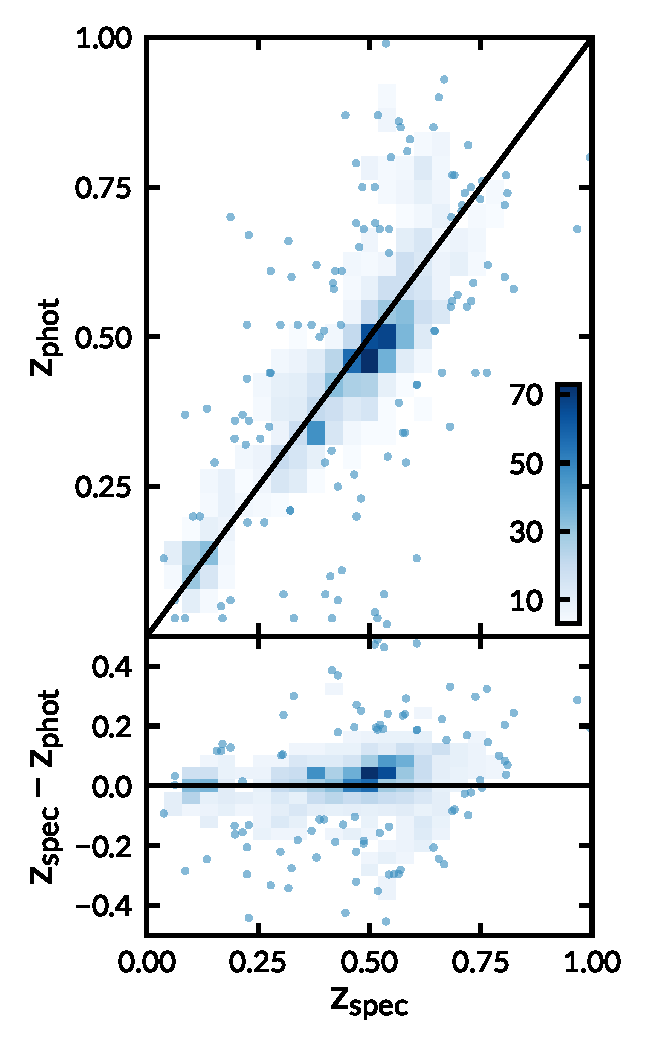
\includegraphics[width=\textwidth]{figures/specVSphot.pdf} 
	\caption{This is a placeholder figure for a figure about how we are doing with the photo-z's. I'm still working out exactly what we should show on the figure, and whether it should be a single or double column figure.} 
	\label{fig:icd_vs_mass} 
\end{figure*}

We assess the effectiveness of our photo-z estimates by comparing with the available spectroscopic redshifts (spec-z) from the SDSS. We use three diagnostics to gauge photo-z accuracy. First, we report the full scatter between the photo-z and spec-z, defined as:
\begin{equation}
	\sigma_f = \mathrm{RMS}[\delta z/(1+z_{spec})]
\end{equation}
where $\delta z = z_{spec} - z_{phot}$. Second, we report the normalized median absolute deviation (NMAD; \citealt{Ilbert2009, Dahlen2013, Molino2017}), given as
\begin{equation}
	\sigma_{NMAD} = 1.48 \times \mathrm{median} \bigg{(} \frac{|\delta z|}{1+z_{spec}} \bigg{)}.
\end{equation}   
which provides an estimate of the scatter resistant to catastrophic outliers. Finally, the catastrophic outlier fraction (OLF) where we define a catastrophic outlier (following \citealt{Molino2017}) as,
\begin{equation}
	\eta = \frac{|\delta z|}{(1+z_{spec})} > 5 \times \sigma_{NMAD}.
\end{equation}


\subsection{Cluster Finding}
We create RGB images using \textsc{stiff} \citep{Bertin2011}. We use \textsc{MaxBCG} \citep{Koester2007b}.

\section{Results and Discussion}\label{sec:results}

Lorem ipsum dolor amet swag copper mug meh tilde, put a bird on it live-edge tattooed kinfolk before they sold out locavore selvage leggings raclette literally bicycle rights. Hot chicken kickstarter mustache vinyl roof party. Wayfarers brooklyn truffaut twee umami, venmo irony. Typewriter viral pop-up, listicle vaporware organic af salvia keytar twee chillwave austin +1 offal blog. La croix dreamcatcher snackwave, try-hard intelligentsia taxidermy messenger bag air plant godard mustache celiac glossier echo park. Photo booth readymade authentic glossier biodiesel snackwave beard hammock sriracha before they sold out edison bulb fixie PBR\&B. Man bun pabst kogi, crucifix subway tile af tacos cray tumeric lyft cronut lomo tattooed.

\section{Summary}\label{sec:summary}

Lorem ipsum dolor amet swag copper mug meh tilde, put a bird on it live-edge tattooed kinfolk before they sold out locavore selvage leggings raclette literally bicycle rights. Hot chicken kickstarter mustache vinyl roof party. Wayfarers brooklyn truffaut twee umami, venmo irony. Typewriter viral pop-up, listicle vaporware organic af salvia keytar twee chillwave austin +1 offal blog. La croix dreamcatcher snackwave, try-hard intelligentsia taxidermy messenger bag air plant godard mustache celiac glossier echo park. Photo booth readymade authentic glossier biodiesel snackwave beard hammock sriracha before they sold out edison bulb fixie PBR\&B. Man bun pabst kogi, crucifix subway tile af tacos cray tumeric lyft cronut lomo tattooed.

\section*{Acknowledgements} This research made use of \textsc{APLpy}, an open-source plotting package for Python hosted at \url{http://aplpy.github.com}; the \textsc{IPython} package \citep{Perez2007}; \textsc{matplotlib}, a Python library for publication quality graphics \citep{Hunter2007}. \textsc{iraf} is distributed by the National Optical Astronomy Observatory, which is operated by the Association of Universities for Research in Astronomy under cooperative agreement with the National Science Foundation \citep{Tody1993}. \textsc{PyRAF} is a product of the Space Telescope Science Institute, which is operated by AURA for NASA. Funding for the SDSS and SDSS-II has been provided by the Alfred P. Sloan Foundation, the Participating Institutions, the National Science Foundation, the U.S. Department of Energy, the National Aeronautics and Space Administration, the Japanese Monbukagakusho, the Max Planck Society, and the Higher Education Funding Council for England. The SDSS Web Site is \url{http://www.sdss.org/}. The SDSS is managed by the Astrophysical Research Consortium for the Participating Institutions. This work has made use of data from the European Space Agency (ESA) mission {\it Gaia} (\url{https://www.cosmos.esa.int/gaia}), processed by the {\it Gaia} Data Processing and Analysis Consortium (DPAC, \url{https://www.cosmos.esa.int/web/gaia/dpac/consortium}). Funding for the DPAC has been provided by national institutions, in particular the institutions participating in the {\it Gaia} Multilateral Agreement.

%%%%%%%%%%%%%%%%%%%% REFERENCES %%%%%%%%%%%%%%%%%%
% The best way to enter references is to use BibTeX:
\bibliographystyle{apj}
\bibliography{master}

% if your bibtex file is called example.bib
%%%%%%%%%%%%%%%%% APPENDICES %%%%%%%%%%%%%%%%%%%%%

\appendix

\section{SWARP}\label{app:swarp}
%\begin{verbatim}
%#----------------------------------- Output -----------------------------------
%IMAGEOUT_NAME          coadd.fits      # Output filename
%WEIGHTOUT_NAME       coadd.weight.fits # Output weight-map filename
%
%HEADER_ONLY            N               # Only a header as an output file (Y/N)?
%HEADER_SUFFIX          .head           # Filename extension for additional headers
%
%#------------------------------- Input Weights --------------------------------
%
%WEIGHT_TYPE            NONE            # BACKGROUND,MAP_RMS,MAP_VARIANCE
%# or MAP_WEIGHT
%WEIGHT_SUFFIX          .weight.fits    # Suffix to use for weight-maps
%WEIGHT_IMAGE                           # Weightmap filename if suffix not used
%# (all or for each weight-map)
%
%#------------------------------- Co-addition ----------------------------------
%
%COMBINE                Y               # Combine resampled images (Y/N)?
%COMBINE_TYPE           MEDIAN          # MEDIAN,AVERAGE,MIN,MAX,WEIGHTED,CHI2
%# or SUM
%
%#-------------------------------- Astrometry ----------------------------------
%
%CELESTIAL_TYPE         NATIVE          # NATIVE, PIXEL, EQUATORIAL,
%# GALACTIC,ECLIPTIC, or SUPERGALACTIC
%PROJECTION_TYPE        TAN             # Any WCS projection code or NONE
%PROJECTION_ERR         0.001           # Maximum projection error (in output
%# pixels), or 0 for no approximation
%CENTER_TYPE            MANUAL             # MANUAL, ALL or MOST
%CENTER         00:00:00.0, +00:00:00.0 # Coordinates of the image center
%PIXELSCALE_TYPE        MANUAL          # MANUAL,FIT,MIN,MAX or MEDIAN
%PIXEL_SCALE            0.2666          # Pixel scale
%IMAGE_SIZE             0               # Image size (0 = AUTOMATIC)
%
%#-------------------------------- Resampling ----------------------------------
%
%RESAMPLE               Y               # Resample input images (Y/N)?
%RESAMPLE_DIR           .               # Directory path for resampled images
%RESAMPLE_SUFFIX        .resamp.fits    # filename extension for resampled images
%
%RESAMPLING_TYPE        LANCZOS3        # NEAREST,BILINEAR,LANCZOS2,LANCZOS3
%# or LANCZOS4 (1 per axis)
%OVERSAMPLING           0               # Oversampling in each dimension
%# (0 = automatic)
%INTERPOLATE            N               # Interpolate bad input pixels (Y/N)?
%# (all or for each image)
%
%FSCALASTRO_TYPE        FIXED           # NONE or FIXED
%FSCALE_KEYWORD         FLXSCALE        # FITS keyword for the multiplicative
%# factor applied to each input image
%FSCALE_DEFAULT         1.0             # Default FSCALE value if not in header
%
%GAIN_KEYWORD           GAIN            # FITS keyword for effect. gain (e-/ADU)
%GAIN_DEFAULT           0.0             # Default gain if no FITS keyword found
%# 0 = infinity (all or for each image)
%
%#--------------------------- Background subtraction ---------------------------
%
%SUBTRACT_BACK          Y               # Subtraction sky background (Y/N)?
%# (all or for each image)
%
%BACK_TYPE              AUTO            # AUTO or MANUAL
%# (all or for each image)
%BACK_DEFAULT           0.0             # Default background value in MANUAL
%# (all or for each image)
%BACK_SIZE              128             # Background mesh size (pixels)
%# (all or for each image)
%BACK_FILTERSIZE        3               # Background map filter range (meshes)
%# (all or for each image)
%
%#------------------------------ Memory management -----------------------------
%
%VMEM_DIR               .               # Directory path for swap files
%VMEM_MAX               2047            # Maximum amount of virtual memory (MB)
%MEM_MAX                128             # Maximum amount of usable RAM (MB)
%COMBINE_BUFSIZE        64              # RAM dedicated to co-addition(MB)
%
%#------------------------------ Miscellaneous ---------------------------------
%
%DELETE_TMPFILES        Y               # Delete temporary resampled FITS files
%# (Y/N)?
%COPY_KEYWORDS          OBJECT          # List of FITS keywords to propagate
%# from the input to the output headers
%WRITE_FILEINFO         N               # Write information about each input
%# file in the output image header?
%WRITE_XML              N               # Write XML file (Y/N)?
%XML_NAME               swarp.xml       # Filename for XML output
%VERBOSE_TYPE           NORMAL          # QUIET,NORMAL or FULL
%
%NTHREADS               0               # Number of simultaneous threads for
%# the SMP version of SWarp
%# 0 = automatic
%\end{verbatim}

\section{SExtractor}\label{app:sextractor}
%\begin{verbatim}
%#-------------------------------- Catalog ------------------------------------
%
%CATALOG_NAME     test.cat       # name of the output catalog
%CATALOG_TYPE     ASCII_HEAD     # NONE,ASCII,ASCII_HEAD, ASCII_SKYCAT,
%# ASCII_VOTABLE, FITS_1.0 or FITS_LDAC
%PARAMETERS_NAME  $PIPE/confs/bcs_Catalog.param  # name of the file containing catalog contents
%
%#------------------------------- Extraction ----------------------------------
%
%DETECT_TYPE      CCD            # CCD (linear) or PHOTO (with gamma correction)
%DETECT_MINAREA   12              # min. # of pixels above threshold
%DETECT_MAXAREA   0              # max. # of pixels above threshold (0=unlimited)
%THRESH_TYPE      RELATIVE       # threshold type: RELATIVE (in sigmas)
%# or ABSOLUTE (in ADUs)
%DETECT_THRESH    1.5            # <sigmas> or <threshold>,<ZP> in mag.arcsec-2
%ANALYSIS_THRESH  1.0            # <sigmas> or <threshold>,<ZP> in mag.arcsec-2
%
%FILTER           Y              # apply filter for detection (Y or N)?
%FILTER_NAME      $PIPE/confs/configs/gauss_3.0_5x5.conv   # name of the file containing the filter
%FILTER_THRESH                   # Threshold[s] for retina filtering
%
%DEBLEND_NTHRESH  32             # Number of deblending sub-thresholds
%DEBLEND_MINCONT  0.005          # Minimum contrast parameter for deblending
%
%CLEAN            Y              # Clean spurious detections? (Y or N)?
%CLEAN_PARAM      1.0            # Cleaning efficiency
%
%MASK_TYPE        CORRECT        # type of detection MASKing: can be one of
%# NONE, BLANK or CORRECT
%
%#-------------------------------- WEIGHTing ----------------------------------
%
%WEIGHT_TYPE      NONE           # type of WEIGHTing: NONE, BACKGROUND,
%# MAP_RMS, MAP_VAR or MAP_WEIGHT
%RESCALE_WEIGHTS  Y              # Rescale input weights/variances (Y/N)?
%WEIGHT_IMAGE     weight.fits    # weight-map filename
%WEIGHT_GAIN      Y              # modulate gain (E/ADU) with weights? (Y/N)
%WEIGHT_THRESH                   # weight threshold[s] for bad pixels
%
%#-------------------------------- FLAGging -----------------------------------
%
%FLAG_IMAGE       flag.fits      # filename for an input FLAG-image
%FLAG_TYPE        OR             # flag pixel combination: OR, AND, MIN, MAX
%# or MOST
%
%#------------------------------ Photometry -----------------------------------
%
%PHOT_APERTURES   11.25              # MAG_APER aperture diameter(s) in pixels
%PHOT_AUTOPARAMS  2.5, 3.5       # MAG_AUTO parameters: <Kron_fact>,<min_radius>
%PHOT_PETROPARAMS 2.0, 3.5       # MAG_PETRO parameters: <Petrosian_fact>,
%# <min_radius>
%PHOT_AUTOAPERS   0.0,0.0        # <estimation>,<measurement> minimum apertures
%# for MAG_AUTO and MAG_PETRO
%PHOT_FLUXFRAC    0.5            # flux fraction[s] used for FLUX_RADIUS
%
%SATUR_LEVEL      50000.0        # level (in ADUs) at which arises saturation
%SATUR_KEY        SATURATE       # keyword for saturation level (in ADUs)
%
%MAG_ZEROPOINT    0.0            # magnitude zero-point
%MAG_GAMMA        4.0            # gamma of emulsion (for photographic scans)
%GAIN             0.0            # detector gain in e-/ADU
%GAIN_KEY         GAIN           # keyword for detector gain in e-/ADU
%PIXEL_SCALE      0.0            # size of pixel in arcsec (0=use FITS WCS info)
%
%#------------------------- Star/Galaxy Separation ----------------------------
%
%SEEING_FWHM      1.2            # stellar FWHM in arcsec
%STARNNW_NAME     $PIPE/confs/configs/default.nnw    # Neural-Network_Weight table filename
%
%#------------------------------ Background -----------------------------------
%
%BACK_TYPE        AUTO           # AUTO or MANUAL
%BACK_VALUE       0.0            # Default background value in MANUAL mode
%BACK_SIZE        64             # Background mesh: <size> or <width>,<height>
%BACK_FILTERSIZE  3              # Background filter: <size> or <width>,<height>
%
%BACKPHOTO_TYPE   GLOBAL         # can be GLOBAL or LOCAL
%BACKPHOTO_THICK  24             # thickness of the background LOCAL annulus
%BACK_FILTTHRESH  0.0            # Threshold above which the background-
%# map filter operates
%
%#------------------------------ Check Image ----------------------------------
%
%CHECKIMAGE_TYPE  NONE           # can be NONE, BACKGROUND, BACKGROUND_RMS,
%# MINIBACKGROUND, MINIBACK_RMS, -BACKGROUND,
%# FILTERED, OBJECTS, -OBJECTS, SEGMENTATION,
%# or APERTURES
%CHECKIMAGE_NAME  check.fits     # Filename for the check-image
%
%#--------------------- Memory (change with caution!) -------------------------
%
%MEMORY_OBJSTACK  3000           # number of objects in stack
%MEMORY_PIXSTACK  300000         # number of pixels in stack
%MEMORY_BUFSIZE   1024           # number of lines in buffer
%
%#------------------------------- ASSOCiation ---------------------------------
%
%ASSOC_NAME       sky.list       # name of the ASCII file to ASSOCiate
%ASSOC_DATA       2,3,4          # columns of the data to replicate (0=all)
%ASSOC_PARAMS     2,3,4          # columns of xpos,ypos[,mag]
%ASSOCCOORD_TYPE  PIXEL          # ASSOC coordinates: PIXEL or WORLD
%ASSOC_RADIUS     2.0            # cross-matching radius (pixels)
%ASSOC_TYPE       NEAREST        # ASSOCiation method: FIRST, NEAREST, MEAN,
%# MAG_MEAN, SUM, MAG_SUM, MIN or MAX
%ASSOCSELEC_TYPE  MATCHED        # ASSOC selection type: ALL, MATCHED or -MATCHED
%
%#----------------------------- Miscellaneous ---------------------------------
%
%VERBOSE_TYPE     NORMAL         # can be QUIET, NORMAL or FULL
%HEADER_SUFFIX    .head          # Filename extension for additional headers
%WRITE_XML        N              # Write XML file (Y/N)?
%XML_NAME         sex.xml        # Filename for XML output
%XSL_URL          file:///opt/sextractor_2.19.5/share/sextractor/sextractor.xsl
%# Filename for XSL style-sheet
%NTHREADS         1              # 1 single thread
%
%FITS_UNSIGNED    N              # Treat FITS integer values as unsigned (Y/N)?
%INTERP_MAXXLAG   16             # Max. lag along X for 0-weight interpolation
%INTERP_MAXYLAG   16             # Max. lag along Y for 0-weight interpolation
%INTERP_TYPE      ALL            # Interpolation type: NONE, VAR_ONLY or ALL
%
%#--------------------------- Experimental Stuff -----------------------------
%
%PSF_NAME         default.psf    # File containing the PSF model
%PSF_NMAX         1              # Max.number of PSFs fitted simultaneously
%PATTERN_TYPE     RINGS-HARMONIC # can RINGS-QUADPOLE, RINGS-OCTOPOLE,
%# RINGS-HARMONICS or GAUSS-LAGUERRE
%SOM_NAME         default.som    # File containing Self-Organizing Map weights
%\end{verbatim}

\end{document}
